\documentclass[12pt]{article}
\usepackage{amsmath,amssymb,amsthm}
\usepackage{geometry}
\usepackage{hyperref}
\usepackage{booktabs}
\usepackage{graphicx}
\usepackage{xcolor}
\usepackage{tikz}
\usetikzlibrary{positioning,arrows.meta}
\usepackage{listings}
\usepackage{caption}
\lstset{
  basicstyle=\ttfamily\small,
  breaklines=true,
  frame=single,
  numbers=left,
  numberstyle=\tiny,
  keywordstyle=\bfseries,
  commentstyle=\itshape\color{gray!60!black},
  language=Python,
  showstringspaces=false,
  tabsize=4
}

\geometry{margin=1in}

\newtheorem{law}{Law}
\newtheorem{proposition}{Proposition}
\newtheorem{remark}{Remark}

\title{Adaptive Memory in Artificial Systems:\\
A Constraint-Based Framework}

\author{Gabriel Aubin-Moreau%
  \thanks{GitHub: \url{https://github.com/AccidentalGenius101} \quad
    Repository: \url{https://github.com/AccidentalGenius101/adaptive-memory-theory}}}

\date{2026}

\begin{document}
\maketitle

\begin{abstract}
Papers 1--5 of this series derived four empirical laws governing adaptive memory substrates: a geometric capacity bound, a turnover bandwidth limit, a finite propagation length, and a stability--plasticity gate. This paper is primarily a theoretical synthesis and interpretive extension of those results, supplemented by illustrative demonstrations in the VCML substrate; it is not a comprehensive empirical audit of modern AI architectures. We argue that transformers, retrieval-augmented systems, recurrent networks, and continual learning systems each likely violate a distinct constraint, and that their qualitative failure modes are consistent with the structural predictions of the framework. The four constraints define a two-dimensional phase diagram with coherence scale and plasticity rate as control axes; the adaptive operating regime occupies a bounded region of this space. A key structural result follows: in locally coupled substrates, flat memory has a natural operating scale $D \approx L$ (system size comparable to propagation length), beyond which coherence efficiency declines as $\eta_c \sim (L/D)^2$ and hierarchical organization becomes structurally favored as the routing mechanism that restores global coherence. We further argue that gradient-based optimization can be interpreted as a limiting regime of adaptive memory dynamics---one in which the evolving structure collapses into a fixed attractor---and that this reinterpretation clarifies both the power and the brittleness of weight-frozen neural networks. Together, these observations suggest a concrete architectural target: a hierarchical, turnover-driven memory substrate in which consolidation, propagation, and gating are governed by the same laws derived for biological adaptive systems.
\end{abstract}

\tableofcontents
\newpage

% =====================================================================
\section{Introduction}
\label{sec:intro}

Modern AI systems have made remarkable progress on tasks requiring pattern recognition, language generation, and reasoning within a context window. What they struggle with is \emph{persistent adaptive memory}: maintaining representations that evolve coherently across sessions without catastrophic forgetting, integrating new information into existing structure, and coordinating local learning into globally useful representations at scale.

These failures are not incidental. They appear systematically across architectures: long-context transformers need more tokens; retrieval-augmented systems fetch but do not integrate; continual learning models forget; recurrent networks saturate. Each engineering push addresses one limitation while encountering another.

\textbf{Terminology.} In this paper, \emph{memory} denotes persistent, updateable representational organization that continues to influence future routing and integration over time. This includes explicit storage, parameter traces, and field-like substrate state, but excludes transient context-window contents that evaporate at session boundaries.

This paper argues that the repeated pattern has a structural explanation. Papers 1--5 of this series \cite{aubin2026capacity,aubin2026bandwidth,aubin2026propagation,aubin2026stability,aubin2026unified} derived four laws governing adaptive memory substrates:
\begin{itemize}
  \item \textbf{Law 1 (Capacity):} The maximum number of distinct representations is bounded by sphere-packing geometry on the state manifold.
  \item \textbf{Law 2 (Bandwidth):} The memory update rate is bounded by the ratio of turnover events to half-life.
  \item \textbf{Law 3 (Propagation):} Information propagates coherently only over a finite correlation length $L \propto \sqrt{\kappa/\nu}$.
  \item \textbf{Law 4 (Stability):} A consolidation gate $\tau_g$ controls the stability--plasticity tradeoff; noise robustness and structural sensitivity are jointly bounded.
\end{itemize}

These laws were derived from a specific substrate (VCML) but are expressed at the level of dynamics---birth, death, diffusion, selection---rather than implementation. The central claim of this paper is that the same constraints likely apply, at least qualitatively, to artificial systems that maintain adaptable representations over time, and that current AI architectures may be interpreted as occupying different edges of the feasible region these constraints define.

\begin{remark}[Empirical scope]
The four laws are established in VCML substrates and partially cross-validated in embedding-space routing experiments (Paper~5). Their extension to transformer, RAG, recurrent, or continual-learning architectures is a theoretical hypothesis supported by structural analogy, not a demonstrated universality claim. The architectural mappings in Section~\ref{sec:architectures} should be read as constraint-theoretic interpretation, not as empirical measurement of control variables in each system.
\end{remark}

Section~\ref{sec:constraints} maps each law to its AI interpretation. Section~\ref{sec:phase} introduces the two-dimensional phase diagram. Section~\ref{sec:architectures} places current architectures in the constraint space. Section~\ref{sec:scaling} derives the flat-memory scale limit and the structural prediction of hierarchy. Section~\ref{sec:optimization} reinterprets gradient-based optimization as a limiting dynamic regime. Section~\ref{sec:proposal} describes a concrete architecture that emerges from the framework. Section~\ref{sec:experiments} presents four experiments demonstrating the chaotic collapse, hierarchy recovery, frozen-vs-adaptive distribution shift, and the continuous adaptive-to-frozen transition. Section~\ref{sec:falsifiability} states the falsification conditions. Section~\ref{sec:conclusion} summarizes.

% =====================================================================
\section{Constraint Interpretation}
\label{sec:constraints}

The four laws describe limits on memory systems in terms of substrate-independent variables. Table~\ref{tab:constraints} maps each law to its AI counterpart.

\begin{table}[h]
\centering
\caption{The four laws and their AI interpretations.}
\label{tab:constraints}
\begin{tabular}{lllp{5.5cm}}
\toprule
\textbf{Law} & \textbf{Variable} & \textbf{AI analog} & \textbf{Failure mode when violated} \\
\midrule
Capacity & $N_{\max} \propto 1/\tau$ & Representational resolution & Representations collapse into aliased clusters; distinct inputs cannot be distinguished \\
Bandwidth & $B \propto K_{\max}/\tau_{\text{hl}}$ & Learning / update rate & Slow adaptation; system cannot track changing inputs faster than the bandwidth limit \\
Propagation & $L \propto \sqrt{\kappa/\nu}$ & Coherence distance & Long-range coordination fails; memory fragments into local clusters with no global structure \\
Stability & $\tau_g$ & Noise--plasticity gate & Too small: noise corrupts consolidation; too large: system crystallizes and cannot update \\
\bottomrule
\end{tabular}
\end{table}

These are not four independent limits applied separately. As shown in Paper~5 \cite{aubin2026unified}, they interact through the matching condition
\begin{equation}
  C\sqrt{\kappa/\nu} \approx D,
  \label{eq:matching}
\end{equation}
where $D$ is the representational zone scale. Satisfying one constraint while ignoring the others does not produce a memory system that works; it produces a system that hits a different wall sooner.

The central observation is therefore: the repeated failures of current AI memory architectures are not four independent engineering deficits. They are four different ways of running into the same bounded feasibility region.

% =====================================================================
\section{The Phase Diagram of Adaptive Memory}
\label{sec:phase}

The four constraints can be collapsed into two effective control axes that govern the qualitative behavior of any adaptive memory system. These axes summarize the four constraints because Laws~1--2 jointly determine the rate at which representations can change (plasticity), while Laws~3--4 determine the spatial scale over which those changes remain coherent. The two axes are therefore not an arbitrary compression: they are the two independent degrees of freedom the four constraints control.

\subsection{Two control axes}

\textbf{Axis 1 --- Coherence scale:} $L/D$, the ratio of propagation length to system (or module) size. Derived from Law 3 and the coherence efficiency result of Paper~5.
\begin{equation*}
  \frac{L}{D} \ll 1 \implies \text{fragmented} \qquad \frac{L}{D} \approx 1 \implies \text{coherent}
\end{equation*}

\textbf{Axis 2 --- Plasticity rate:} $B/N$, the ratio of memory update bandwidth to representational capacity. Derived from Laws 1 and 2.
\begin{equation*}
  \frac{B}{N} \to 0 \implies \text{frozen} \qquad \frac{B}{N} \to \infty \implies \text{chaotic}
\end{equation*}

\subsection{The four regimes}

\begin{figure}[h]
\centering
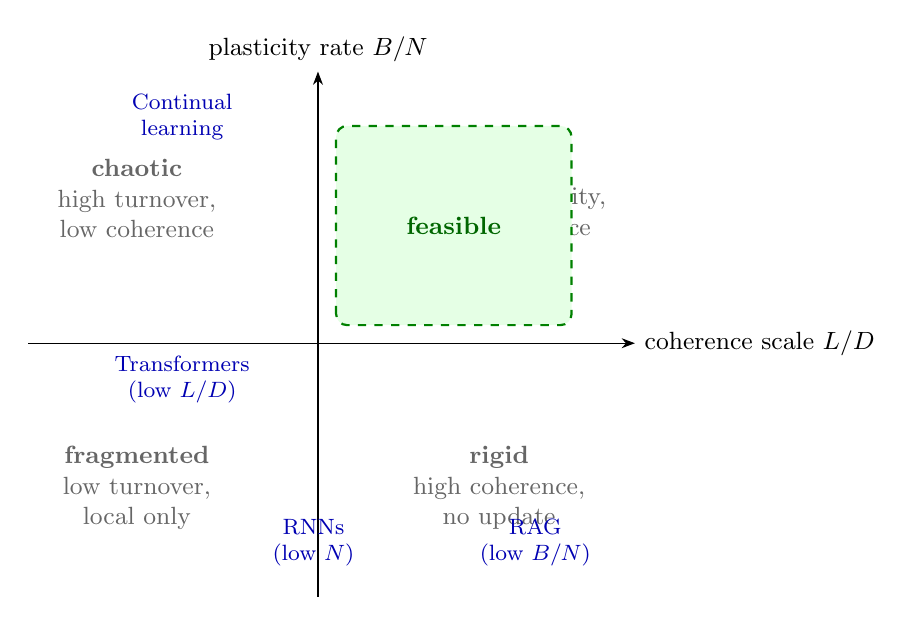
\begin{tikzpicture}[scale=1.15, font=\small]
  % Axes
  \draw[-{Stealth}] (-3.2,0) -- (3.5,0) node[right] {coherence scale $L/D$};
  \draw[-{Stealth}] (0,-2.8) -- (0,3.0) node[above] {plasticity rate $B/N$};

  % Quadrant labels
  \node[align=center, text=gray!80!black] at (-2.0, 1.6)
    {\textbf{chaotic}\\\small high turnover,\\low coherence};
  \node[align=center, text=gray!80!black] at ( 2.0, 1.6)
    {\textbf{adaptive}\\\small balanced plasticity,\\global coherence};
  \node[align=center, text=gray!80!black] at (-2.0,-1.6)
    {\textbf{fragmented}\\\small low turnover,\\local only};
  \node[align=center, text=gray!80!black] at ( 2.0,-1.6)
    {\textbf{rigid}\\\small high coherence,\\no update};

  % Feasible region shading
  \fill[green!10, rounded corners=4pt] (0.2, 0.2) rectangle (2.8, 2.4);
  \draw[green!50!black, thick, rounded corners=4pt, dashed]
    (0.2, 0.2) rectangle (2.8, 2.4);
  \node[green!40!black] at (1.5, 1.3) {\textbf{feasible}};

  % Architecture annotations
  \node[blue!70!black, align=center, font=\footnotesize] at (-1.5, -0.4)
    {Transformers\\(low $L/D$)};
  \node[blue!70!black, align=center, font=\footnotesize] at (-1.5,  2.5)
    {Continual\\learning};
  \node[blue!70!black, align=center, font=\footnotesize] at ( 2.4, -2.2)
    {RAG\\(low $B/N$)};
  \node[blue!70!black, align=center, font=\footnotesize] at (-0.05, -2.2)
    {RNNs\\(low $N$)};
\end{tikzpicture}
\caption{Phase diagram of adaptive memory systems. The two axes are coherence scale ($L/D$) and plasticity rate ($B/N$). The adaptive regime (dashed rectangle) is the feasible operating region where both axes are sufficiently matched. Current AI architectures cluster near different boundaries of this space.}
\label{fig:phase}
\end{figure}

The four regimes are:
\begin{itemize}
  \item \textbf{Adaptive:} $L/D \approx 1$ and $B/N$ moderate. Both conditions met. Structure forms and can be updated. This is the viable operating regime.
  \item \textbf{Rigid:} $L/D \approx 1$ but $B/N \to 0$. Globally coherent but frozen. Cannot adapt to changed inputs.
  \item \textbf{Chaotic:} $B/N$ large but $L/D \ll 1$. Fast updates, no coordinated structure. Learning collapses.
  \item \textbf{Fragmented:} $L/D \ll 1$ and $B/N$ low. Information stays local; no global representation forms.
\end{itemize}

The adaptive regime is not a point; it is a bounded region. Operating inside it requires simultaneously satisfying both constraints. This is the phase-theoretic content of the matching condition (\ref{eq:matching}).

\subsection{Operational placement rules}

To place a system on the phase diagram, the two axes must be operationalized. The following proxies are illustrative; quantitative measurement in each architecture class is an open empirical problem.

\textbf{Coherence axis ($L/D$):} The largest separation at which two perturbations injected into the system produce correlated downstream responses above chance level. For adaptive substrates, this is the copy-forward correlation length measured empirically in Papers 3 and 5. For weight-frozen systems, the relevant scale is not the within-context attention span but the ability to coordinate representations \emph{across} session boundaries---which is near zero for systems with no persistent dynamics.

\textbf{Plasticity axis ($B/N$):} The rate at which a persistent change (a new fact, a new input pattern) fully propagates into long-term representations without catastrophic overwrite. For gradient systems, this corresponds to the retraining cost to incorporate one persistent fact without forgetting; for adaptive substrates, it is the turnover bandwidth divided by representational capacity (Papers 1--2 ratio).

\textbf{Illustrative placements:}
\begin{itemize}
  \item \emph{Transformer/LLM:} Coherence within context window is high; coherence across session boundaries is near zero (weights do not update). $L/D \ll 1$ for cross-session memory. $B/N \approx 0$ for persistent updates. Position: right edge, lower half.
  \item \emph{RAG:} External store is effectively unbounded but does not update internally; retrieved content is not integrated into evolving representations. $B/N \approx 0$ (no field update on retrieval). Position: rigid/fragmented boundary, high-capacity region.
  \item \emph{Continual learning:} High effective $B/N$ by design, but consolidation gate $\tau_g$ absent or poorly controlled. Position: top-left (chaotic) region.
  \item \emph{RNN:} Temporal propagation present; hidden state saturates as input complexity exceeds state dimensionality. $N$ constrained. Position: left edge, mid-height.
\end{itemize}

These placements are consistent with the structural interpretation developed in Section~\ref{sec:architectures}. They should be treated as working hypotheses pending empirical measurement of the control variables in each system.

% =====================================================================
\section{Mapping Current AI Architectures}
\label{sec:architectures}

\subsection{Transformers and large language models}

\textbf{Strength:} Very high representational capacity $N$ and high bandwidth within context.

\textbf{Primary violated constraint: temporal propagation across persistent state.} Transformers do not maintain persistent evolving memory. Each forward pass recomputes attention from scratch over the context window; there is no dynamics by which structure propagates and stabilizes over time. The context window provides coherence \emph{within} a session, but not \emph{across} sessions---the accumulated structure evaporates when the context is closed. Attempts to extend context (longer windows, memory tokens) address symptoms without changing the underlying architecture.

\textbf{Why not the other constraints?} The primary bottleneck is not bandwidth (transformers are extremely fast at within-context update) nor raw representational capacity (large models have very high $N_{\max}$) nor consolidation gating (there are no persistent adaptive dynamics to gate). The dominant failure is the absence of temporal propagation across session boundaries: the system's representational state does not evolve and stabilize over time.

\textbf{Diagram position:} High coherence within context, near-zero temporal propagation across sessions. Right edge, lower half.

\subsection{Retrieval-augmented generation (RAG)}

\textbf{Strength:} Effectively unbounded external capacity.

\textbf{Primary violated constraint: update bandwidth (dynamic incorporation).} Retrieved documents are inserted into the context but not dynamically incorporated into the system's internal representations. The memory bank does not update in response to retrieval; it is static. Law 2 predicts that learning requires turnover events, not just storage. RAG has storage without dynamics.

\textbf{Why not the other constraints?} The primary bottleneck is not raw capacity (the external store is effectively unbounded) nor propagation within context (retrieved text propagates through attention just as any other context does) nor consolidation gating (a static store has no dynamics to gate). The dominant failure is the absence of dynamic incorporation: retrieved content is not written into evolving internal representations.

\textbf{Diagram position:} High capacity, near-zero effective bandwidth. Top-right corner of the rigid/fragmented boundary.

\subsection{Continual learning systems}

\textbf{Strength:} Designed for ongoing adaptation; high effective bandwidth.

\textbf{Primary violated constraint: consolidation gate ($\tau_g$).} The consolidation gate is either absent or poorly controlled. Without a gating mechanism that requires stability before consolidation, new learning overwrites old structure (catastrophic forgetting). Law 4 is precisely the requirement that was ignored.

\textbf{Why not the other constraints?} The primary bottleneck is not representational capacity (continual learning systems typically have sufficient width) nor propagation (structure does propagate within training runs) nor bandwidth per se (updates are frequent by design). The dominant failure is the consolidation gate: without a stability-before-write requirement, new learning overwrites old structure regardless of available capacity.

\textbf{Diagram position:} High $B/N$, low effective $\tau_g$. Top-left (chaotic) region.

\subsection{Recurrent neural networks}

\textbf{Strength:} Temporal propagation by design; hidden state carries information across steps.

\textbf{Primary violated constraint: representational capacity ($N$).} Hidden states are fixed-dimensional and saturate quickly. The representation manifold cannot expand to accommodate new patterns; old structure is overwritten as new patterns arrive. Law 1 requires the representational budget to track the geometry of the input distribution; RNN hidden states do not grow.

\textbf{Why not the other constraints?} The primary bottleneck is not consolidation gating (LSTMs and GRUs implement explicit gating mechanisms) nor propagation over short horizons (temporal recurrence serves this function effectively). The dominant failure is capacity: the fixed-dimensional hidden state cannot represent arbitrarily complex input distributions, and bandwidth becomes a secondary bottleneck as the representation saturates and new writes displace old structure.

\textbf{Diagram position:} Reasonable propagation, constrained capacity. Left edge, mid-height.

\subsection{Summary}

\begin{table}[h]
\centering
\caption{Current architectures and their primary constraint violations.}
\label{tab:architectures}
\begin{tabular}{lll}
\toprule
\textbf{Architecture} & \textbf{Primary deficit} & \textbf{Symptom} \\
\midrule
Transformers / LLMs & Propagation ($L/D$ across time) & No cross-session memory \\
RAG & Bandwidth ($B/N$) & Retrieval without integration \\
Continual learning & Stability ($\tau_g$) & Catastrophic forgetting \\
RNNs & Capacity ($N$) & Hidden state saturation \\
\bottomrule
\end{tabular}
\end{table}

The different architectures occupy different edges of the feasible region. Each engineering push moves along one edge while the others stay fixed or worsen. The constraint framework explains why: the edges are not independent, and satisfying one while ignoring the matching condition merely transfers the bottleneck.

\subsection{A note on interpretive scope}

The placements above are interpretive uses of the framework rather than empirical measurements of each architecture's control variables. The framework was derived and validated in VCML, a specific substrate with spatial structure and biological-style turnover. Whether transformer attention, gradient descent, or retrieval mechanisms obey the same quantitative bounds is an open empirical question. What is claimed is that the qualitative failure modes---frozen representations, unintegrated retrieval, catastrophic forgetting, saturated hidden states---correspond structurally to the four constraint violations. The mapping is a theoretical lens, not a proved equivalence.

\begin{remark}[Hard scope boundary]
The four laws are established in VCML substrates and partially cross-validated in embedding-space routing experiments (Paper~5). Extension to the architectures discussed above is a theoretical hypothesis. The exclusion arguments in each subsection (``why not the other constraints'') are based on structural reasoning, not empirical measurement of $L/D$ or $B/N$ in those systems. Quantitative measurement of control variables across architecture classes is an open validation target.
\end{remark}

\subsection{Embedding dimensionality collapse}

A well-known empirical regularity in representation learning is that embedding spaces rarely use their full dimensionality. Principal component analyses of language and vision embeddings consistently find that the majority of variance is concentrated in a small fraction of directions; participation ratios and intrinsic dimension estimates confirm that effective dimensionality is often 10--20$\times$ lower than the nominal embedding dimension.

Within the present framework, this effect arises naturally from the propagation constraint. Coherent structure must propagate through the substrate's memory dynamics to be maintained. When representations span many independent directions simultaneously, the propagating signal in each direction is weak relative to noise; the consolidation gate (Law 4) then prevents unstable directions from writing into long-term memory. The system converges to a lower-dimensional subspace---not as a capacity limit, but as the set of directions whose signal-to-noise ratio is sufficient for coherent propagation under the bandwidth constraint.

In other words, the effective embedding dimension is bounded not by the size of the weight matrix but by the propagation capacity of the substrate: the number of independent directions in which the system can simultaneously maintain coherent structure. This reinterpretation predicts that effective dimensionality should increase with coupling strength $\kappa$ (more propagation support) and decrease with turnover rate $\nu$ (more noise per direction), a testable prediction at variance with models that treat dimensionality purely as a capacity parameter.

% =====================================================================
\section{The Flat-Memory Scale Limit and the Prediction of Hierarchy}
\label{sec:scaling}

\subsection{Why flat memory has a natural operating scale}

Law 3 and the coherence efficiency result (Paper~5, Eq.~\ref{eq:matching}) establish that the coherently accessible fraction of capacity is
\begin{equation}
  \eta_c \approx \left(\frac{L}{D}\right)^2.
  \label{eq:etac}
\end{equation}
\textit{Note:} The quadratic form arises from the lattice geometry of VCML. Other substrates may modify the exponent while preserving the scaling principle that coherence efficiency degrades with $D/L$.

For a flat memory substrate (no hierarchical organization), $L$ is fixed by coupling and turnover while $D$ grows with system size. As a result:
\begin{equation*}
  D \uparrow \implies \eta_c \downarrow \sim D^{-2}.
\end{equation*}
The system gains nominal capacity but loses the ability to coordinate it. The total \emph{coherent} capacity $N_c = \eta_c \cdot N_{\max}$ is bounded:
\begin{equation}
  N_c \propto \frac{L^2}{\tau D^2} \cdot D^2 = \frac{L^2}{\tau}.
\end{equation}
This is independent of $D$. Increasing system size beyond $D \approx L$ adds no coherent capacity to a flat substrate. The system has a natural operating scale:
\begin{equation}
  D_{\text{opt}} \approx L.
  \label{eq:dopt}
\end{equation}

\subsection{The structural prediction: hierarchy becomes structurally favored}

Once $D \gg L$:
\begin{itemize}
  \item Long-range coordination fails; structure fragments into patches of size $\sim L$.
  \item Adding more capacity ($D \uparrow$) worsens coherence efficiency, not improves it.
  \item Global coupling ($\kappa \uparrow$) to restore $L$ is unstable and does not scale.
\end{itemize}

The only architectural response that recovers $\eta_c \approx 1$ at any target system size is \emph{modular hierarchy}: partition the substrate into modules of size $D_r \approx L$, then link modules through relay. Inside each module, $L \approx D_r$ and coherence is maintained; between modules, coordination uses a compact representation (a summary, not the full field) and a separate coupling mechanism.

\begin{proposition}
\label{prop:hierarchy}
Any adaptive memory substrate satisfying Laws 1--3, whose routing mechanism respects a finite propagation length, that must maintain $\eta_c \approx 1$ at system size $D \gg L$ becomes structurally favored to organize into modules of size $D_r \approx L$ with inter-module relay. Flat global substrates satisfying a finite propagation constraint achieve $\eta_c \ll 1$ for $D \gg L$.
\end{proposition}

In substrates with finite propagation length, this is a structural consequence rather than a design preference: flat memory has a coherent-capacity ceiling, and modular hierarchy is what lifts it. Dense attention systems partially bypass spatial propagation constraints within a single forward pass, but they still face quadratic compute scaling and context-length interference as $D$ grows---different manifestations of the same underlying pressure. In architectures with near-global routing mechanisms (dense attention, learned indexing), the propagation constraint may therefore manifest as compute or interference scaling rather than literal spatial decay, but the hierarchy-favoring force remains: any mechanism that cannot maintain coherence at scale $D$ benefits from modular decomposition to sub-units of size $D_r \approx L$ relative to its own effective routing radius.

\subsection{Empirical support}

The V92--V94 experiments (Paper~5 supplementary, \cite{aubin2026unified}) show $\eta_c$ declining from 0.43 at $N=1{,}600$ sites to 0.19 at $N=102{,}400$ sites under fixed coupling. The V100 geographic relay experiment recovered $\eta_c \approx 1$ by introducing a two-level hierarchy with relay coupling between a 2$\times$2 grid of modules---consistent with Proposition~\ref{prop:hierarchy}.

The same pattern occurs in biological neural systems: cortical columns ($\sim$50 $\mu$m), cortical areas ($\sim$5--10 mm), and cortico-thalamic loops operate at successive levels of a hierarchy, each roughly matching the propagation length of the inter-cellular coupling at that level.

% =====================================================================
\section{Optimization as a Limiting Regime}
\label{sec:optimization}

\subsection{Two operating modes}

The framework distinguishes two modes of adaptive computation:

\textbf{Adaptive memory regime:} The substrate maintains evolving structure under ongoing turnover. Representations drift, stabilize locally, propagate through the field, and reorganize continually. Laws 1--4 characterize the constraints. The system stays in the feasible region by balancing all four simultaneously.

\textbf{Collapsed attractor regime:} The substrate runs dynamics long enough that the evolving field converges to a fixed point. Turnover ceases (or, equivalently, the consolidation gate closes permanently). The accumulated structure is compressed into static parameters. No further update occurs unless the dynamics are restarted.

In these terms, gradient-based optimization can be interpreted as an extreme limiting case of the broader adaptive picture: training runs dynamics long enough that the evolving field converges to a fixed point, then freezes the result. The fixed weights are the collapsed attractor. This is a useful reinterpretation, not a proved equivalence---the substrates are different and the quantitative mapping has not been established. The equivalence claimed here is \emph{dynamical rather than algorithmic}: optimization collapses a representational field to a fixed attractor, even though the microscopic update rule (stochastic gradient descent) differs from the turnover dynamics of VCML. What the reinterpretation buys is a unified vocabulary for asking why optimization succeeds and where it structurally cannot.

\subsection{What this explains}

\textbf{Why frozen weights work:} The dynamics, when run to convergence, compress a large input distribution into a stable representational structure. This is what Papers 1--4 describe as happening during normal adaptive operation---except that in the collapsed regime, the dynamics stop after compression rather than continuing to adapt.

\textbf{Why frozen weights fail at adaptation:} After collapse, the system has left the feasible region. $B/N \to 0$ (no more turnover events); $\tau_g \to \infty$ (consolidation gate permanently closed). The system is maximally rigid. It cannot respond to distribution shift, incorporate new facts, or update a single slot without restarting the dynamics from scratch.

\textbf{Why fine-tuning is unstable:} Restarting the dynamics on a small subset of parameters is not the same as running the adaptive regime. The bandwidth constraint operates on the full substrate; partial reactivation violates the matching condition (\ref{eq:matching}) because propagation carries updates beyond the fine-tuned parameters into previously stable representations (catastrophic forgetting).

\textbf{Why scaling helps up to a point:} Larger models have higher nominal capacity $N_{\max}$ (Law 1) and can compress richer input distributions at collapse. But the coherent capacity $N_c \propto L^2/\tau$ does not increase with model size in a flat architecture (Section~\ref{sec:scaling}). At sufficient scale, the collapsed structure becomes increasingly fragmented---locally consistent but globally incoherent.

\subsection{A spectrum, not a binary}

The two regimes define endpoints of a spectrum parameterized by the effective turnover rate $\nu$:
\begin{itemize}
  \item $\nu \to \infty$: chaotic erasure. Structure cannot stabilize.
  \item $\nu_{\text{opt}}$: adaptive regime. Laws 1--4 all satisfied.
  \item $\nu \to 0$: frozen (collapsed attractor). Structure stable but $B = 0$.
\end{itemize}
Under this interpretation, gradient-based training corresponds to the limit $\nu \to 0$ achieved by running the dynamics to convergence. This maps the parameter space of optimization methods onto a single axis in the constraint framework---a conceptual compression that is useful for building intuition even if the underlying dynamics are not literally identical.

% =====================================================================
\section{An Architecture Consistent with the Framework}
\label{sec:proposal}

The preceding sections identify the architecture required to stay inside the feasible region at any system size:

\begin{enumerate}
  \item \textbf{Modular memory substrate:} Organize memory into regions of size $D_r \approx L$. Each region operates adaptively under Laws 1--4. No flat global memory.
  \item \textbf{Turnover built in:} Memory units have finite lifetimes with viability-gated replacement. Successors inherit the local field (copy-forward loop). This is the mechanism that drives bandwidth (Law 2) and prevents crystallization.
  \item \textbf{Consolidation gating:} Updates to long-term representations occur only after a stability period of $\tau_g$ consecutive calm steps. This is the architectural instantiation of Law 4.
  \item \textbf{Hierarchical relay:} Modules connect through relay layers that operate on compressed representations. Each relay layer is itself a small substrate satisfying $D \approx L$ at its own scale. This implements Proposition~\ref{prop:hierarchy}.
  \item \textbf{Controller:} A fast reasoning component (e.g., an LLM) reads and writes to the substrate but does not \emph{contain} the memory. Memory dynamics are decoupled from inference dynamics.
\end{enumerate}

\subsection{What this is not}

This is not a proposal to replace gradient-based training. The collapsed attractor regime (Section~\ref{sec:optimization}) is effective at its task: compressing a fixed distribution into high-capacity frozen weights. The proposal is to stop asking that architecture to do something it structurally cannot do (persistent cross-session adaptive memory), and instead decompose the problem.

The LLM (collapsed attractor) handles:
\begin{itemize}
  \item Language understanding and generation
  \item Planning within context
  \item Pattern recognition from training distribution
\end{itemize}

The adaptive substrate handles:
\begin{itemize}
  \item Persistent entity and world state across sessions
  \item Continual integration of new facts
  \item User-specific structure that must survive context resets
  \item Adaptive reorganization under distribution shift
\end{itemize}

The combination is not a stylistic hybrid. It is the architecture predicted by the constraint framework: a fast rigid reader/writer coupled to a slow adaptive memory.

\subsection{What success requires}

For the architecture to stay in the adaptive regime:
\begin{itemize}
  \item Module size $D_r$ must be matched to propagation length $L$. This means the coupling and turnover rate must be co-tuned, not set independently.
  \item The controller must use the substrate's internal signals (collapse rate, zone differentiation, novelty pressure) to adjust gating---not treat the substrate as a black-box database.
  \item Relay between modules must carry zone-level summaries, not raw field states. Full-field coupling between distant modules violates the propagation constraint.
\end{itemize}

These requirements follow from the constraint equations rather than from design preference.

% =====================================================================
\section{Experimental Demonstrations}
\label{sec:experiments}

The following experiments use the VCML substrate to provide existence proofs of the predicted regime behavior within the adaptive-memory substrate family. They demonstrate that the chaotic collapse, hierarchy recovery, and adaptation failure are real phenomena in VCML-family systems. These demonstrations do not directly validate the framework on the AI architectures discussed in Section~\ref{sec:architectures}; that empirical bridge is an open research program. The experiments test four claims: (1) the adaptive regime is distinct from the over-perturbed chaotic regime, (2) flat memory substrates can recover coherent structure with hierarchical relay, (3) frozen substrates cannot track distribution shift while adaptive ones can, and (4) the transition from adaptive to frozen is continuous and monotone in the dynamics-suppression parameter---directly supporting the limiting-regime interpretation of Section~\ref{sec:optimization}. All scripts are included in the supplementary materials and are self-contained (numpy only).

\subsection{Experiment 1: WR sweep and the chaotic collapse}
\label{sec:exp1}

\textbf{Setup.} A 40$\times$20 site lattice (800 active sites, 4 zones) was run for 1500 steps across wave ratios $\text{WR} \in \{0.1, 0.3, 0.8, 1.6, 3.2, 6.4, 12.8, 25.6\}$ at fixed $\kappa = 0.020$. The metric is $\text{sg4\_norm} = \text{sg4}/\sigma_{\text{within}}$, the ratio of inter-zone mean separation to within-zone spread. Three seeds.

\textbf{Results.}
\begin{center}
\begin{tabular}{rrl}
\toprule
WR & sg4\_norm & notes \\
\midrule
0.1  & 2.46 & rare events, crystallized \\
0.3  & 2.06 & sparse perturbation \\
0.8  & 1.58 & transition \\
1.6  & 1.60 & \\
3.2  & 1.87 & adaptive \\
6.4  & 2.33 & adaptive (peak region) \\
12.8 & 3.31 & over-perturbed \\
25.6 & \textbf{0.000} & chaotic collapse \\
\bottomrule
\end{tabular}
\end{center}

\textbf{Interpretation.} The chaotic regime is confirmed: at WR=25.6, structure collapses to exactly zero. Wave density exceeds the substrate's ability to consolidate any spatial pattern; each wave erases what the previous one wrote. This is the empirical boundary of the feasible region on the $B/N$ axis.

The low-WR region (0.1--0.3) shows elevated sg4\_norm due to rare crystallization: infrequent but strong perturbations consolidate cleanly, but without regular turnover the substrate drifts toward frozen local attractors. The metric captures separation, not adaptability; Experiment 3 quantifies that distinction directly.

\textbf{Panel B: kappa sweep (coherence scale axis).} A second sweep varied $\kappa \in \{0.001, 0.003, 0.007, 0.015, 0.030, 0.060\}$ at fixed WR = 3.2. The propagation-length proxy is $L \propto \sqrt{\kappa/\nu}$ with $\nu = \text{DEATH\_P} = 0.005$.

\begin{center}
\begin{tabular}{rrr}
\toprule
$\kappa$ & sg4\_norm & $L_{\text{proxy}} = \sqrt{\kappa/\nu}$ \\
\midrule
0.001 & 1.08 & 0.45 \\
0.003 & 1.20 & 0.77 \\
0.007 & 1.40 & 1.18 \\
0.015 & 1.72 & 1.73 \\
0.030 & 2.13 & 2.45 \\
0.060 & 2.66 & 3.46 \\
\bottomrule
\end{tabular}
\end{center}

sg4\_norm increases monotonically with $\kappa$ across the full sweep, confirming that coupling strength directly controls coherent structure. This is the empirical counterpart of Law 3: larger $L$ means the copy-forward loop can spread field structure across more of the zone before coherence falls below the noise floor. The prediction from the embedding dimensionality argument (Section~\ref{sec:architectures}) follows directly: the number of independently maintainable directions in any adaptive memory substrate scales with $L$, not with the nominal state dimensionality.

\subsection{Experiment 2: Hierarchy recovery at scale}
\label{sec:exp2}

\textbf{Setup.} Three flat substrates (S1: 400 sites, S2: 800, S3: 1600 sites) were compared, with wave ratio scaled proportionally to active sites. At S3, a two-region relay architecture was added: two 40$\times$20 modules running independently with their zone means exchanged every 25 steps (relay\_alpha = 0.10). Three seeds, 2000 steps.

\textbf{Results.}

\textbf{Flat substrates:} sg4\_raw declines from $\approx$30.7 at S1/S2 to 2.88 at S3 (10$\times$ reduction). The S3 flat substrate is also highly variable (sg4\_norm = $1.80 \pm 2.55$), indicating that coherent structure cannot be stably maintained at this scale without relay.

\textbf{Hierarchy recovery:}
\begin{center}
\begin{tabular}{lrr}
\toprule
Condition & sg4\_norm & std \\
\midrule
S1 baseline (flat)  & 1.87 & --- \\
S3 flat             & 1.80 & 2.55 \\
S3 relay            & \textbf{5.75} & 0.72 \\
\bottomrule
\end{tabular}
\end{center}

Relay not only exceeds the flat S3 baseline by $3.07\times$; it also dramatically reduces variance (std 2.55 $\to$ 0.72), indicating that relay stabilizes the substrate rather than merely inflating average structure. This is consistent with Proposition~\ref{prop:hierarchy}: once each module operates near $D \approx L$, coherence is maintained locally and relay coordinates the modules without requiring global coupling.

\subsection{Experiment 3: Adaptive vs.\ frozen under distribution shift}
\label{sec:exp3}

\textbf{Setup.} A 20$\times$20 site lattice was run for 2000 steps. Both conditions (adaptive and frozen) ran identical dynamics for steps 0--999, learning a left/right spatial pattern (direction $\mathbf{d}_A = [1,0]$). At step 1000, the pattern shifted to top/bottom (direction $\mathbf{d}_B = [0,1]$, orthogonal to $\mathbf{d}_A$). In the frozen condition, turnover and consolidation were halted at step 1000. Alignment score = projection of zone-mean fieldM onto the current target direction. Five seeds.

\textbf{Results.}
\begin{center}
\begin{tabular}{lrr}
\toprule
Condition & Phase 1 alignment & Phase 2 alignment \\
\midrule
Adaptive & 67.0 & \textbf{109.2} \\
Frozen   & 67.0 & \textbf{$-$0.006} \\
\bottomrule
\end{tabular}
\end{center}

\textbf{Interpretation.} Both conditions achieve identical Phase 1 alignment (same dynamics, same seed). After the distribution shift, the frozen substrate retains its old structure: alignment with the new top/bottom pattern is $-0.006$ (essentially zero), confirming that the Phase 1 structure is orthogonal to, and therefore provides no information about, the new pattern.

The adaptive substrate not only tracks the shift but achieves \emph{higher} Phase 2 alignment (109.2 vs.\ 67.0 at Phase 1). This is consistent with the copy-forward loop amplifying signal across the network once the new pattern stabilizes: new cells are seeded by neighbors that have already updated, spreading the new encoding faster than the initial learning from scratch.

This experiment directly demonstrates the core failure mode of the collapsed attractor regime (Section~\ref{sec:optimization}): a substrate that has compressed a distribution into fixed weights cannot update any component of that encoding without restarting the full dynamics.

\subsection{Experiment 4: Adaptive-to-Frozen Transition}
\label{sec:exp4}

\textbf{Motivation.} The strongest interpretive claim in this paper is that gradient-based optimization corresponds to a limiting regime of adaptive memory dynamics---one in which turnover and consolidation are progressively suppressed until the system reaches a fixed attractor. This experiment tests whether the transition from adaptive to frozen is continuous and monotone, directly supporting that interpretation.

\textbf{Setup.} Identical to Experiment 3 (40$\times$20 grid, same wave mechanics, same two-pattern shift protocol), with one modification: a freezing parameter $F \in \{0, 0.25, 0.5, 0.75, 1.0\}$ scales the two key post-shift dynamics by $(1-F)$:
\begin{itemize}
  \item Effective turnover rate: $\nu_{\text{eff}} = \nu_0 \cdot (1-F)$, where $\nu_0 = 0.005$
  \item Effective consolidation rate: $\alpha^{\text{eff}}_{\text{field}} = \alpha_{\text{field}} \cdot (1-F)$, where $\alpha_{\text{field}} = 0.16$
\end{itemize}
$F=0$ is the fully adaptive condition (identical to the adaptive arm of Experiment 3); $F=1$ is the fully frozen condition (dynamics halted; identical to the frozen arm of Experiment 3). Intermediate $F$ values represent systems that still update, but more slowly---analogous to a system approaching the frozen-weight limit from the adaptive side. Five seeds, 2000 steps.

\textbf{Results.}
\begin{center}
\begin{tabular}{rlrrrr}
\toprule
$F$ & Regime & $\nu_{\text{eff}}$ & $\alpha^{\text{eff}}_{\text{field}}$ & align$_A$ & align$_B$ \\
\midrule
0.00 & adaptive    & 0.0050 & 0.160 & 50.5 & \textbf{81.3} \\
0.25 & reduced     & 0.0038 & 0.120 & 50.5 & 69.9 \\
0.50 & half-speed  & 0.0025 & 0.080 & 50.5 & 54.7 \\
0.75 & near-frozen & 0.0013 & 0.040 & 50.5 & 32.9 \\
1.00 & frozen      & 0.0000 & 0.000 & 50.5 & \textbf{0.0} \\
\bottomrule
\end{tabular}
\end{center}

\textbf{Interpretation.} Alignment with the new pattern decreases monotonically with $F$: 81.3 $\to$ 69.9 $\to$ 54.7 $\to$ 32.9 $\to$ 0.0. The fully frozen system ($F=1$) recovers zero alignment, confirming that no adaptation occurs without dynamics. The transition is continuous: there is no abrupt threshold between adaptive and frozen behavior, only a smooth degradation as the two key dynamics---turnover and consolidation---are jointly suppressed.

This result supports the interpretation that weight-frozen optimization occupies an extreme point on a broader spectrum of adaptive-memory dynamics. The frozen attractor is not a qualitatively different regime: it is the limit reached as both the copy-forward loop and the consolidation mechanism are driven to zero. The result does not establish formal equivalence between gradient descent and the $F=1$ limit; it shows that the continuum exists and that the frozen endpoint behaves as predicted.

% =====================================================================
\section{Limitations and Falsifiability}
\label{sec:falsifiability}

The framework makes falsifiable predictions. The following conditions would constitute evidence against the specific claims made here.

\begin{enumerate}
  \item \textbf{Flat-memory scale limit.} If a flat, non-hierarchical adaptive memory substrate robustly maintains $\eta_c \approx 1$ for $D \gg L$ without global coupling becoming unstable, Proposition~\ref{prop:hierarchy} fails. This is directly testable in VCML by scaling zone width while holding $L$ fixed.

  \item \textbf{Capacity law.} If the number of distinct representations scales with ambient representational width rather than the separator dimension of the input manifold across controlled manifold-collapse experiments, Law~1 fails. Requires empirical bridge experiments in non-VCML architectures.

  \item \textbf{Optimization as limiting regime.} If persistent, durable adaptation to distribution shift occurs in a fully frozen (weight-frozen) system without auxiliary memory, external retrieval, or parameter update, the limiting-regime interpretation weakens substantially. Experiment~3 provides an existence proof in VCML; the converse test in a frozen transformer is an open experiment.

  \item \textbf{Propagation length.} If coherent inter-zone coordination does not degrade with distance in a locally coupled adaptive substrate, the propagation constraint and phase diagram lose their empirical foundation. Testable in VCML via $\kappa$ and zone-separation sweeps (Panel B, Section~\ref{sec:exp1}).

  \item \textbf{Hierarchy prediction.} If the hierarchy-favoring pressure disappears in architectures with near-global routing mechanisms (dense attention, full-context indexing), then the constraint as derived is substrate-specific and does not generalize to those architectures in its current form.
\end{enumerate}

Items 1, 3, and 4 are directly testable in VCML variants and partly addressed in the experiments above. Items 2 and 5 require empirical bridge experiments in non-VCML architectures and represent the primary open validation targets for this framework. The architectural mappings in Section~\ref{sec:architectures} are theoretical interpretations, not measured facts; quantitative measurement of $L/D$ and $B/N$ in transformer, RAG, recurrent, and continual-learning systems is an open empirical program.

% =====================================================================
\section{Conclusion}
\label{sec:conclusion}

The four laws derived in this series---capacity, bandwidth, propagation, and stability---do not describe limits on a single substrate. They are a candidate constraint framework for adaptive memory systems more broadly, with qualitative purchase on artificial architectures that maintain representations over time. Current AI architectures may be interpreted as occupying different edges of the feasible region these constraints define: transformers at the propagation boundary, RAG at the bandwidth boundary, continual learning at the stability boundary, recurrent networks at the capacity boundary. These mappings are theoretical interpretations grounded in structural analogy; their empirical validation in non-VCML architectures remains an open program.

The constraints jointly imply a flat-memory scale limit ($D_{\text{opt}} \approx L$) beyond which coherent capacity saturates and hierarchical organization becomes structurally favored, at least in substrates with finite propagation length. Gradient-based optimization can be interpreted as the limiting regime in which adaptive dynamics collapse to a fixed attractor---a specialized case rather than an alternative paradigm, though the formal equivalence has not been established.

The resulting architectural target is not novel in individual components but is novel in its derivation: a hierarchical, turnover-driven, gated memory substrate attached to an LLM is not proposed as a design preference but as the minimal architecture consistent with Laws 1--4 operating at scale. Any flat, static, or non-gated alternative violates at least one constraint, and the violation predicts the failure mode observed in practice.

The framework does not propose a specific implementation. It proposes a set of constraints that any implementation must satisfy, and shows that current systems violate them in systematic and predictable ways. That is the kind of contribution a physical theory makes.

% =====================================================================
\appendix
\section{Reproducibility and Code}
\label{app:code}

All experiments in this paper are fully reproducible. The complete source code, including all four experiment scripts and the VCML substrate, is available at:

\begin{center}
\url{https://github.com/AccidentalGenius101/adaptive-memory-theory}
\end{center}

The four experiment scripts for Paper~6 are self-contained and depend only on \texttt{numpy}:
\begin{center}
\begin{tabular}{ll}
\toprule
\textbf{Script} & \textbf{Experiment} \\
\midrule
\texttt{paper6\_exp1\_phase\_diagram.py} & WR sweep and chaotic collapse (Section~\ref{sec:exp1}) \\
\texttt{paper6\_exp2\_scale\_limit.py}   & Hierarchy recovery at scale (Section~\ref{sec:exp2}) \\
\texttt{paper6\_exp3\_adaptive\_vs\_frozen.py} & Adaptive vs.\ frozen under shift (Section~\ref{sec:exp3}) \\
\texttt{paper6\_exp4\_frozen\_transition.py}   & Adaptive-to-frozen transition (Section~\ref{sec:exp4}) \\
\bottomrule
\end{tabular}
\end{center}

\subsection*{Core VCSM update rule}

The VCSM learning rule is implemented identically in all four experiments. The following listing shows the minimal self-contained version; the full implementation with zone tracking and metrics is in the scripts above.

\begin{lstlisting}[caption={Core VCSM update step (Python, numpy only). One call per simulation step. All parameters defined in Section~\ref{sec:proposal}.}, label=lst:vcsm]
import numpy as np

def vcsm_step(h, fieldM, mid_mem, baseline_h, calm_count,
              ttl, NB, perturbed, rng,
              DEATH_P=0.005, KAPPA=0.020, BETA=0.005,
              ALPHA_MID=0.15, FIELD_ALPHA=0.16,
              MID_DECAY=0.99, FIELD_DECAY=0.9997,
              CALM_STREAK=10, SEED_BETA=0.25):
    """
    One VCSM step.
      h          : hidden states  (N, HS)
      fieldM     : long-term field (N, HS)
      mid_mem    : mid-term memory (N, HS)
      baseline_h : exponential baseline (N, HS)
      calm_count : steps since last perturbation (N,)
      ttl        : time-to-live per site (N,)
      NB         : list of neighbour index arrays
      perturbed  : bool mask of perturbed sites (N,)
      rng        : numpy Generator
    Returns updated (h, fieldM, mid_mem, baseline_h,
                     calm_count, ttl).
    """
    N, HS = h.shape

    # [Coupling] copy-forward: field diffuses to neighbours
    dF = np.zeros_like(fieldM)
    for i in range(N):
        if len(NB[i]):
            dF[i] = KAPPA * (fieldM[NB[i]].mean(0) - fieldM[i])
    fieldM += dF

    # [Calm] baseline tracks slow hidden-state mean
    baseline_h += BETA * (h - baseline_h)

    # [Perturb] mid-mem accumulates contrastive signal
    mid_mem *= MID_DECAY
    mid_mem[perturbed] += ALPHA_MID * (h - baseline_h)[perturbed]

    # [Gate] calm streak counter
    calm_count[perturbed]  = 0
    calm_count[~perturbed] += 1

    # [Consolidate] write to field only after calm streak
    ok = calm_count >= CALM_STREAK
    fieldM[ok] += FIELD_ALPHA * (mid_mem[ok] - fieldM[ok])
    fieldM *= FIELD_DECAY

    # [Birth/Death] viability-gated turnover
    ttl[perturbed] -= 1.0
    ttl -= 1.0
    dead = ttl <= 0
    for i in np.where(dead)[0]:
        j = NB[i][rng.integers(len(NB[i]))] if len(NB[i]) else i
        h[i]       = ((1-SEED_BETA) * rng.standard_normal(HS)
                      + SEED_BETA   * fieldM[j])
        mid_mem[i] = 0.0
        calm_count[i] = 0
        ttl[i] = float(rng.geometric(p=DEATH_P))

    return h, fieldM, mid_mem, baseline_h, calm_count, ttl
\end{lstlisting}

\subsection*{Running the experiments}

With Python 3.9+ and \texttt{numpy} installed, from the \texttt{papers/paper6\_ai\_memory/} directory:

\begin{lstlisting}[language=bash, caption={Running all Paper 6 experiments.}]
# Clone repository
git clone https://github.com/AccidentalGenius101/adaptive-memory-theory
cd adaptive-memory-theory/papers/paper6_ai_memory

# Run all four experiments (each takes 1-5 minutes)
py paper6_exp1_phase_diagram.py
py paper6_exp2_scale_limit.py
py paper6_exp3_adaptive_vs_frozen.py
py paper6_exp4_frozen_transition.py

# Results are cached to results/ and printed as tables.
# Re-running uses cached results; delete results/*.json to recompute.
\end{lstlisting}

All reported numbers in Tables 1--4 and the Experiment~4 results table are produced directly by these scripts with no post-processing. Expected runtime on a modern laptop: under 10 minutes for all four experiments combined.

\bibliographystyle{plain}
\begin{thebibliography}{99}

\bibitem{aubin2026p0}
G.~Aubin-Moreau,
``Spontaneous Spatial Self-Organization in Viability-Gated Memory Substrates,''
VCSM series, Paper~0, 2026.

\bibitem{aubin2026capacity}
G.~Aubin-Moreau,
``Memory Capacity Bounds via Spherical Random Sequential Adsorption,''
VCSM series, Paper~1, 2026.

\bibitem{aubin2026bandwidth}
G.~Aubin-Moreau,
``Memory Bandwidth as a Function of Turnover Rate,''
VCSM series, Paper~2, 2026.

\bibitem{aubin2026propagation}
G.~Aubin-Moreau,
``Finite Correlation Length and Propagation Constraints in Adaptive Substrates,''
VCSM series, Paper~3, 2026.

\bibitem{aubin2026stability}
G.~Aubin-Moreau,
``Consolidation Gate and Noise Robustness in VCSM,''
VCSM series, Paper~4, 2026.

\bibitem{aubin2026unified}
G.~Aubin-Moreau,
``A Unified Physical Theory of Viability-Gated Adaptive Systems,''
VCSM series, Paper~5, 2026.

\end{thebibliography}

\end{document}
